\documentclass[14pt]{extbook}
\usepackage{multicol, enumerate, enumitem, hyperref, color, soul, setspace, parskip, fancyhdr} %General Packages
\usepackage{amssymb, amsthm, amsmath, latexsym, units, mathtools} %Math Packages
\everymath{\displaystyle} %All math in Display Style
% Packages with additional options
\usepackage[headsep=0.5cm,headheight=12pt, left=1 in,right= 1 in,top= 1 in,bottom= 1 in]{geometry}
\usepackage[usenames,dvipsnames]{xcolor}
\usepackage{dashrule}  % Package to use the command below to create lines between items
\newcommand{\litem}[1]{\item#1\hspace*{-1cm}\rule{\textwidth}{0.4pt}}
\pagestyle{fancy}
\lhead{Makeup Progress Quiz 3}
\chead{}
\rhead{Version B}
\lfoot{1648-1753}
\cfoot{}
\rfoot{Summer C 2021}
\begin{document}

\begin{enumerate}
\litem{
Solve the quadratic equation below. Then, choose the intervals that the solutions $x_1$ and $x_2$ belong to, with $x_1 \leq x_2$.\[ 20x^{2} +69 x + 54 = 0 \]\begin{enumerate}[label=\Alph*.]
\item \( x_1 \in [-45.52, -43.94] \text{ and } x_2 \in [-24.15, -23.84] \)
\item \( x_1 \in [-2.64, -1.75] \text{ and } x_2 \in [-1.36, -1.19] \)
\item \( x_1 \in [-6.99, -6.27] \text{ and } x_2 \in [-0.45, -0.38] \)
\item \( x_1 \in [-9.98, -8.56] \text{ and } x_2 \in [-0.34, -0.25] \)
\item \( x_1 \in [-4.51, -2.44] \text{ and } x_2 \in [-0.85, -0.68] \)

\end{enumerate} }
\litem{
Factor the quadratic below. Then, choose the intervals that contain the constants in the form $(ax+b)(cx+d); b \leq d.$\[ 54x^{2} +75 x + 25 \]\begin{enumerate}[label=\Alph*.]
\item \( a \in [1.5, 3.2], \hspace*{5mm} b \in [2, 8], \hspace*{5mm} c \in [17.6, 18.16], \text{ and } \hspace*{5mm} d \in [1, 7] \)
\item \( a \in [0.4, 1.1], \hspace*{5mm} b \in [29, 37], \hspace*{5mm} c \in [-0.37, 1.43], \text{ and } \hspace*{5mm} d \in [42, 50] \)
\item \( a \in [23.8, 28.5], \hspace*{5mm} b \in [2, 8], \hspace*{5mm} c \in [1.52, 4.76], \text{ and } \hspace*{5mm} d \in [1, 7] \)
\item \( a \in [6.8, 10.1], \hspace*{5mm} b \in [2, 8], \hspace*{5mm} c \in [5.08, 7.07], \text{ and } \hspace*{5mm} d \in [1, 7] \)
\item \( \text{None of the above.} \)

\end{enumerate} }
\litem{
Graph the equation below.\[ f(x) = -(x+4)^2 + 19 \]\begin{enumerate}[label=\Alph*.]
\begin{multicols}{2}\item 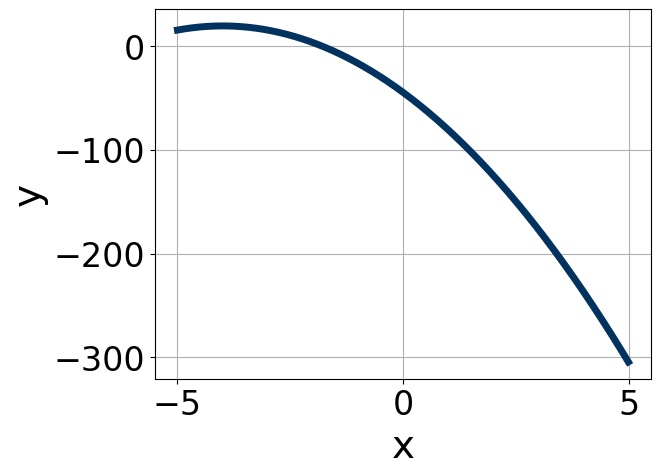
\includegraphics[width = 0.3\textwidth]{../Figures/quadraticEquationToGraphAB.png}\item 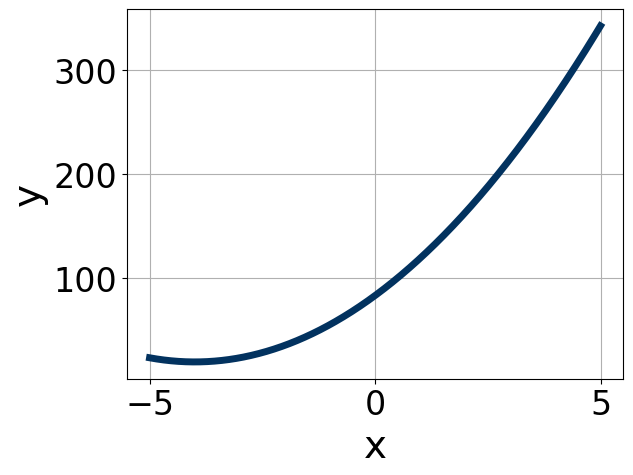
\includegraphics[width = 0.3\textwidth]{../Figures/quadraticEquationToGraphBB.png}\item 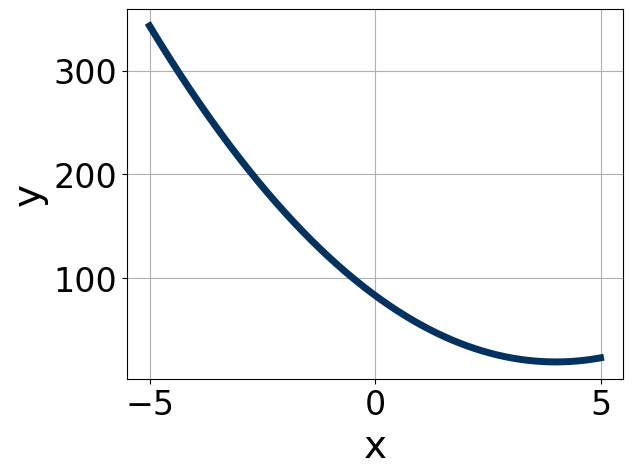
\includegraphics[width = 0.3\textwidth]{../Figures/quadraticEquationToGraphCB.png}\item 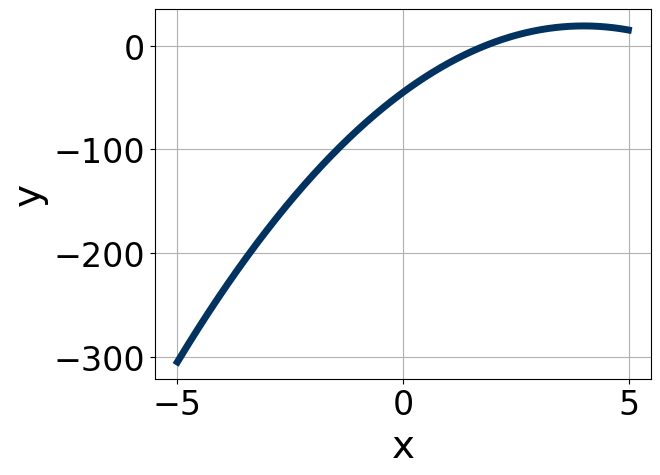
\includegraphics[width = 0.3\textwidth]{../Figures/quadraticEquationToGraphDB.png}\end{multicols}\item None of the above.
\end{enumerate} }
\litem{
Factor the quadratic below. Then, choose the intervals that contain the constants in the form $(ax+b)(cx+d); b \leq d.$\[ 36x^{2} -53 x + 10 \]\begin{enumerate}[label=\Alph*.]
\item \( a \in [-2.4, 2.2], \hspace*{5mm} b \in [-50, -41], \hspace*{5mm} c \in [0.8, 1.6], \text{ and } \hspace*{5mm} d \in [-9, -4] \)
\item \( a \in [-2.4, 2.2], \hspace*{5mm} b \in [-5, 0], \hspace*{5mm} c \in [24.3, 30.5], \text{ and } \hspace*{5mm} d \in [-4, 2] \)
\item \( a \in [1.6, 5.8], \hspace*{5mm} b \in [-5, 0], \hspace*{5mm} c \in [6.7, 9.1], \text{ and } \hspace*{5mm} d \in [-4, 2] \)
\item \( a \in [7.1, 8.5], \hspace*{5mm} b \in [-5, 0], \hspace*{5mm} c \in [2.8, 4.5], \text{ and } \hspace*{5mm} d \in [-4, 2] \)
\item \( \text{None of the above.} \)

\end{enumerate} }
\litem{
Write the equation of the graph presented below in the form $f(x)=ax^2+bx+c$, assuming  $a=1$ or $a=-1$. Then, choose the intervals that $a, b,$ and $c$ belong to.
\begin{center}
    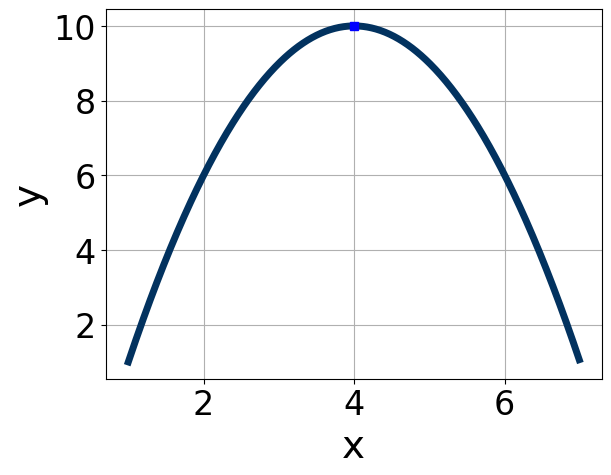
\includegraphics[width=0.5\textwidth]{../Figures/quadraticGraphToEquationCopyB.png}
\end{center}
\begin{enumerate}[label=\Alph*.]
\item \( a \in [-5, 0], \hspace*{5mm} b \in [-9, -7], \text{ and } \hspace*{5mm} c \in [-26, -24] \)
\item \( a \in [0, 3], \hspace*{5mm} b \in [-9, -7], \text{ and } \hspace*{5mm} c \in [25, 28] \)
\item \( a \in [-5, 0], \hspace*{5mm} b \in [-9, -7], \text{ and } \hspace*{5mm} c \in [-6, -4] \)
\item \( a \in [-5, 0], \hspace*{5mm} b \in [4, 10], \text{ and } \hspace*{5mm} c \in [-6, -4] \)
\item \( a \in [0, 3], \hspace*{5mm} b \in [4, 10], \text{ and } \hspace*{5mm} c \in [25, 28] \)

\end{enumerate} }
\litem{
Solve the quadratic equation below. Then, choose the intervals that the solutions belong to, with $x_1 \leq x_2$ (if they exist).\[ 17x^{2} +7 x -8 = 0 \]\begin{enumerate}[label=\Alph*.]
\item \( x_1 \in [-15.77, -15.22] \text{ and } x_2 \in [8.53, 9.44] \)
\item \( x_1 \in [-1, -0.62] \text{ and } x_2 \in [-0.21, 0.71] \)
\item \( x_1 \in [-0.7, -0.43] \text{ and } x_2 \in [0.88, 1.7] \)
\item \( x_1 \in [-24.66, -24.53] \text{ and } x_2 \in [23.87, 25.46] \)
\item \( \text{There are no Real solutions.} \)

\end{enumerate} }
\litem{
Solve the quadratic equation below. Then, choose the intervals that the solutions belong to, with $x_1 \leq x_2$ (if they exist).\[ -20x^{2} -15 x + 6 = 0 \]\begin{enumerate}[label=\Alph*.]
\item \( x_1 \in [-27.23, -26.85] \text{ and } x_2 \in [25.7, 27.9] \)
\item \( x_1 \in [-5.88, -5.01] \text{ and } x_2 \in [20.7, 22.9] \)
\item \( x_1 \in [-1.21, -0.87] \text{ and } x_2 \in [0.1, 0.9] \)
\item \( x_1 \in [-0.94, 0.48] \text{ and } x_2 \in [0.7, 2.1] \)
\item \( \text{There are no Real solutions.} \)

\end{enumerate} }
\litem{
Solve the quadratic equation below. Then, choose the intervals that the solutions $x_1$ and $x_2$ belong to, with $x_1 \leq x_2$.\[ 15x^{2} -8 x -16 = 0 \]\begin{enumerate}[label=\Alph*.]
\item \( x_1 \in [-12.36, -11.71] \text{ and } x_2 \in [19.62, 20.69] \)
\item \( x_1 \in [-1.05, -0.61] \text{ and } x_2 \in [0.85, 1.75] \)
\item \( x_1 \in [-4.54, -3.69] \text{ and } x_2 \in [0.24, 0.3] \)
\item \( x_1 \in [-0.66, -0.34] \text{ and } x_2 \in [2.05, 2.76] \)
\item \( x_1 \in [-2.03, -1.49] \text{ and } x_2 \in [0.35, 0.69] \)

\end{enumerate} }
\litem{
Write the equation of the graph presented below in the form $f(x)=ax^2+bx+c$, assuming  $a=1$ or $a=-1$. Then, choose the intervals that $a, b,$ and $c$ belong to.
\begin{center}
    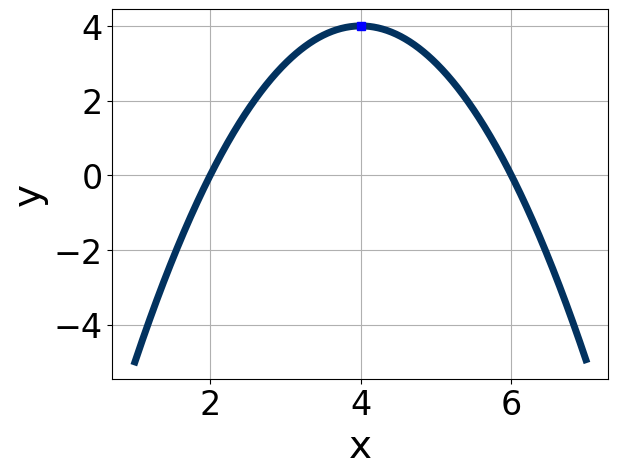
\includegraphics[width=0.5\textwidth]{../Figures/quadraticGraphToEquationB.png}
\end{center}
\begin{enumerate}[label=\Alph*.]
\item \( a \in [-2, 0.2], \hspace*{5mm} b \in [7, 9], \text{ and } \hspace*{5mm} c \in [-12, -8] \)
\item \( a \in [-2, 0.2], \hspace*{5mm} b \in [-13, -7], \text{ and } \hspace*{5mm} c \in [-12, -8] \)
\item \( a \in [0.7, 1.1], \hspace*{5mm} b \in [-13, -7], \text{ and } \hspace*{5mm} c \in [18, 23] \)
\item \( a \in [0.7, 1.1], \hspace*{5mm} b \in [7, 9], \text{ and } \hspace*{5mm} c \in [18, 23] \)
\item \( a \in [-2, 0.2], \hspace*{5mm} b \in [-13, -7], \text{ and } \hspace*{5mm} c \in [-21, -17] \)

\end{enumerate} }
\litem{
Graph the equation below.\[ f(x) = -(x+3)^2 - 16 \]\begin{enumerate}[label=\Alph*.]
\begin{multicols}{2}\item 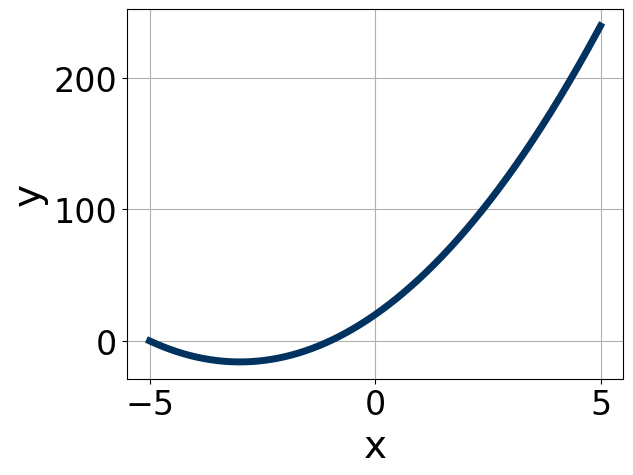
\includegraphics[width = 0.3\textwidth]{../Figures/quadraticEquationToGraphCopyAB.png}\item 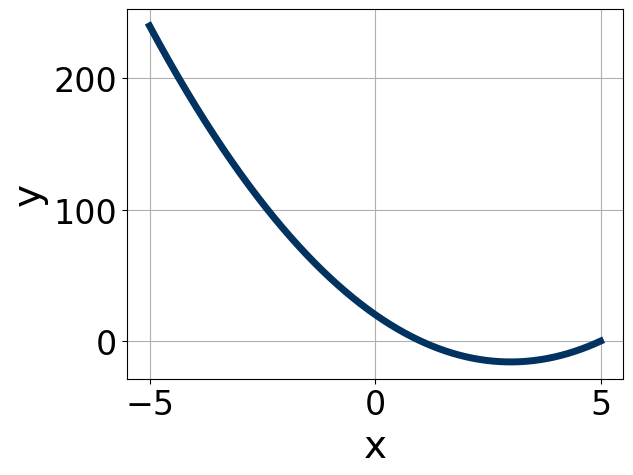
\includegraphics[width = 0.3\textwidth]{../Figures/quadraticEquationToGraphCopyBB.png}\item 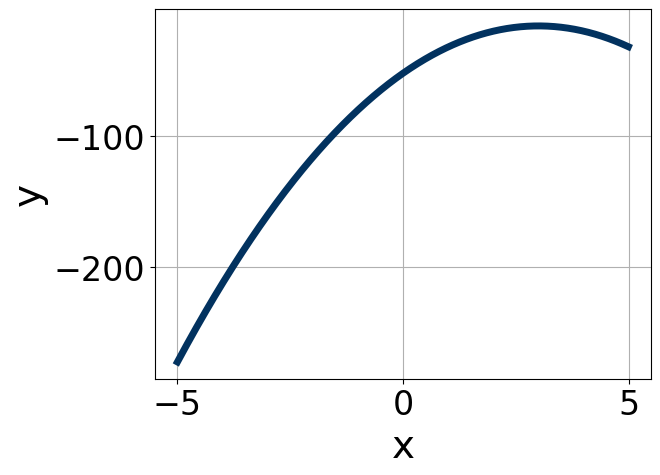
\includegraphics[width = 0.3\textwidth]{../Figures/quadraticEquationToGraphCopyCB.png}\item 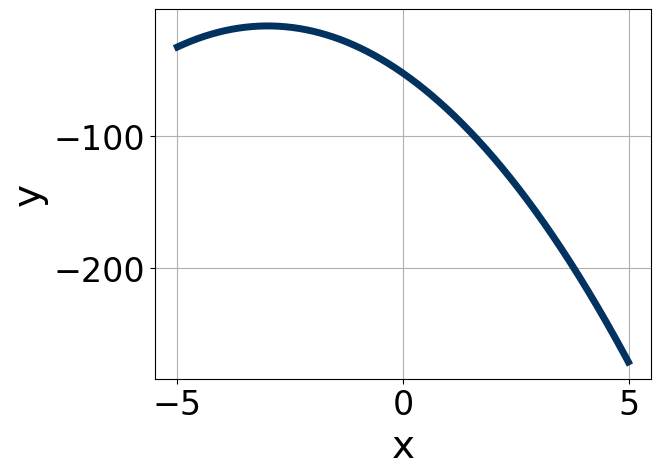
\includegraphics[width = 0.3\textwidth]{../Figures/quadraticEquationToGraphCopyDB.png}\end{multicols}\item None of the above.
\end{enumerate} }
\end{enumerate}

\end{document}